%(i) The extent to which the proposed project methodology is meritorious, including consideration of the extent to which: (A) The proposed project shows awareness of the state-of-the-art for current, related products. (B) The proposed project employs appropriate concepts, components, or systems to develop the new or improved product. (C) The proposed project employs appropriate samples in tests, trials, and other development activities. (D) The proposed project conducts development activities in appropriate environment(s). (E) Input from individuals with disabilities and other key stakeholders is obtained to establish and guide proposed development activities. (F) The applicant identifies and justifies the stage(s) of development for the proposed project; and activities associated with each stage. 

\subsubsection{Background and State of the Art}

Two significant factors impact how effective tactile maps are as tools for enhancing spatial understanding: what information is contained on the map and what tactile symbols are used. 

\textbf{What tactile symbols to use}
The majority of tactile mapmakers are orientation and mobility specialists, typically employed through special education programs
\cite{lobben2012tactile}, \ac{Rowell and Ungar 2003c}. While this implies they are experts in the needs and limitations of people with visual impairments, formal training in cartographic design is limited. There have been some efforts to codify and standardize symbology for tactile maps, however the work has been scattered and there does not yet seem to be a consensus in adoption. Additionally, as illustrated by the annals of graphic map history, there is no guarantee that standardization will result in good maps. Tools produced by mediators limit the agency afforded by the opportunity to dictate one’s own priorities and are susceptible to biases in terms of what information is presented and how that is prioritized. 

In 2012 researchers from the University of Oregon published a comprehensive set of tactile map graphic symbols.  This standard was adopted by the Braille Authority of North America (BANA), to be distributed in their tactile graphics publication
\cite{lobben2012tactile}. However, to date, the only documents available on the BANA’s website predate Lobben and Lawrence’s publication, and thus do not include these proposed standards. In our development, we intend to use this as our reference tactile symbol standard.

\textbf{What information to include}

We consider what information ought to be represented in a tactile map that needs to include the most pertinent information for Deaf-blind individuals to travel in the street environment. Sidewalks are at the heart of traveling through urban centers with low or no vision, and sidewalks support transitions between nearly all other travel options. While having accessible infrastructure such as Tactile Accessible Pedestrian Signals (APS that include a tactile plate rather than only auditory cues) is clearly necessary, knowing of the location of infrastructure (and obstacles) can be equally so. Though we cannot make all sidewalks accessible overnight, foreknowledge of avoidable obstacles aids independent and empowered pedestrian travel.

However, with typical map data (from both proprietary and open sources) it is not currently possible to give a Deaf-blind person an updated tactile map representation that is a relevant, reliable, current record of pedestrian paths accessible to them to or from any location due to a lack of data about the walking environment.  
There are no major digital mapping services to date with a comprehensive sidewalk dataset (\ac{Apple 2019 , Microsoft  2019, Google 2019, OpenStreetMap 2019}). Many cities have made attempts at collecting this data, willingly or otherwise, but disparate efforts, risk being outdated before they begin and often are done in such an imprecise manner that significant clean up needs to be done before the data can be utilized for routing, or other applications that require a finer granularity of data \ac{(Bolten et al. 2016)}. 

Our preliminary studies showed us that this informational gap forces Deaf-blind individuals to risk exploring unverified routes that may strand them in dangerous situations, or abandon independent travel to unknown locations altogether. Furthermore, due to the lack of data and mechanisms, it is not currently possible to systematically ascertain what obstacles exist on a given path, and therefore this social inequality is largely hidden from public view.

\subsubsection{Previous Development}

The OpenSidewalks Project is a data project for the standardized detailed description and appropriate data collection of sidewalk infrastructure.
OpenSidewalks represents a collaboration of data scientists, tool developers, urban specialists, open data communities, educational software specialists, and local advocacy groups, all of whom work to promote equitable and resilient accessible cities.
OpenSidewalks is led by the Taskar Center for Accessible Technology (TCAT) at the University of Washington, who is a project partner.

Our prior work in the OpenSidewalks project defined a data standard for describing the pedestrian environment and the pedestrian network. OpenSidewalks promotes equity in pedestrian routes by making sidewalks first-class members of an open data transportation network \cite{bolten2017}. Collecting open sidewalk information supports a variety of use cases and downstream activities, including addressing the informational gap for pedestrians of all abilities, automated trip planning customized to individual abilities, and furnishing rich analytic tools for data-driven urban planning. 

In order to facilitate the end goal, the OpenSidewalks project focused on employing open source, crowd contributed, geospatial data from OpenStreetMap (OSM). OpenStreetMap was chosen for its extensive global coverage and easily extendable data schema. This platform allows for the project to easily pull from a large existing data pool, while also making it simple enough to fill in informational gaps as they pertain to pedestrians. For inclusion of updated transit data, OSM is also an appropriate platform choice since it is designed to include support for updated transportation data from fixed-route services (GTFS feeds) \cite{OpenStreetMap}.

There are many aspects of the pedestrian environment that we consider for inclusion in pre-optimized tangible map tiles for people who are Deaf-blind.  Based on our pilot focus groups and informational interviews, we incorporated \textit{surfaces}, \textit{topography} and \textit{street interfaces} into our own published data standard described by OpenSidewalks; these critical features promote wayfinding, mobility and safety for people with a range of visual capacities. Figure \ref{fig:DataFeatures} demonstrate the features of a surface that were evaluated for inclusion in the maps. 

\begin{figure}
    \centering
    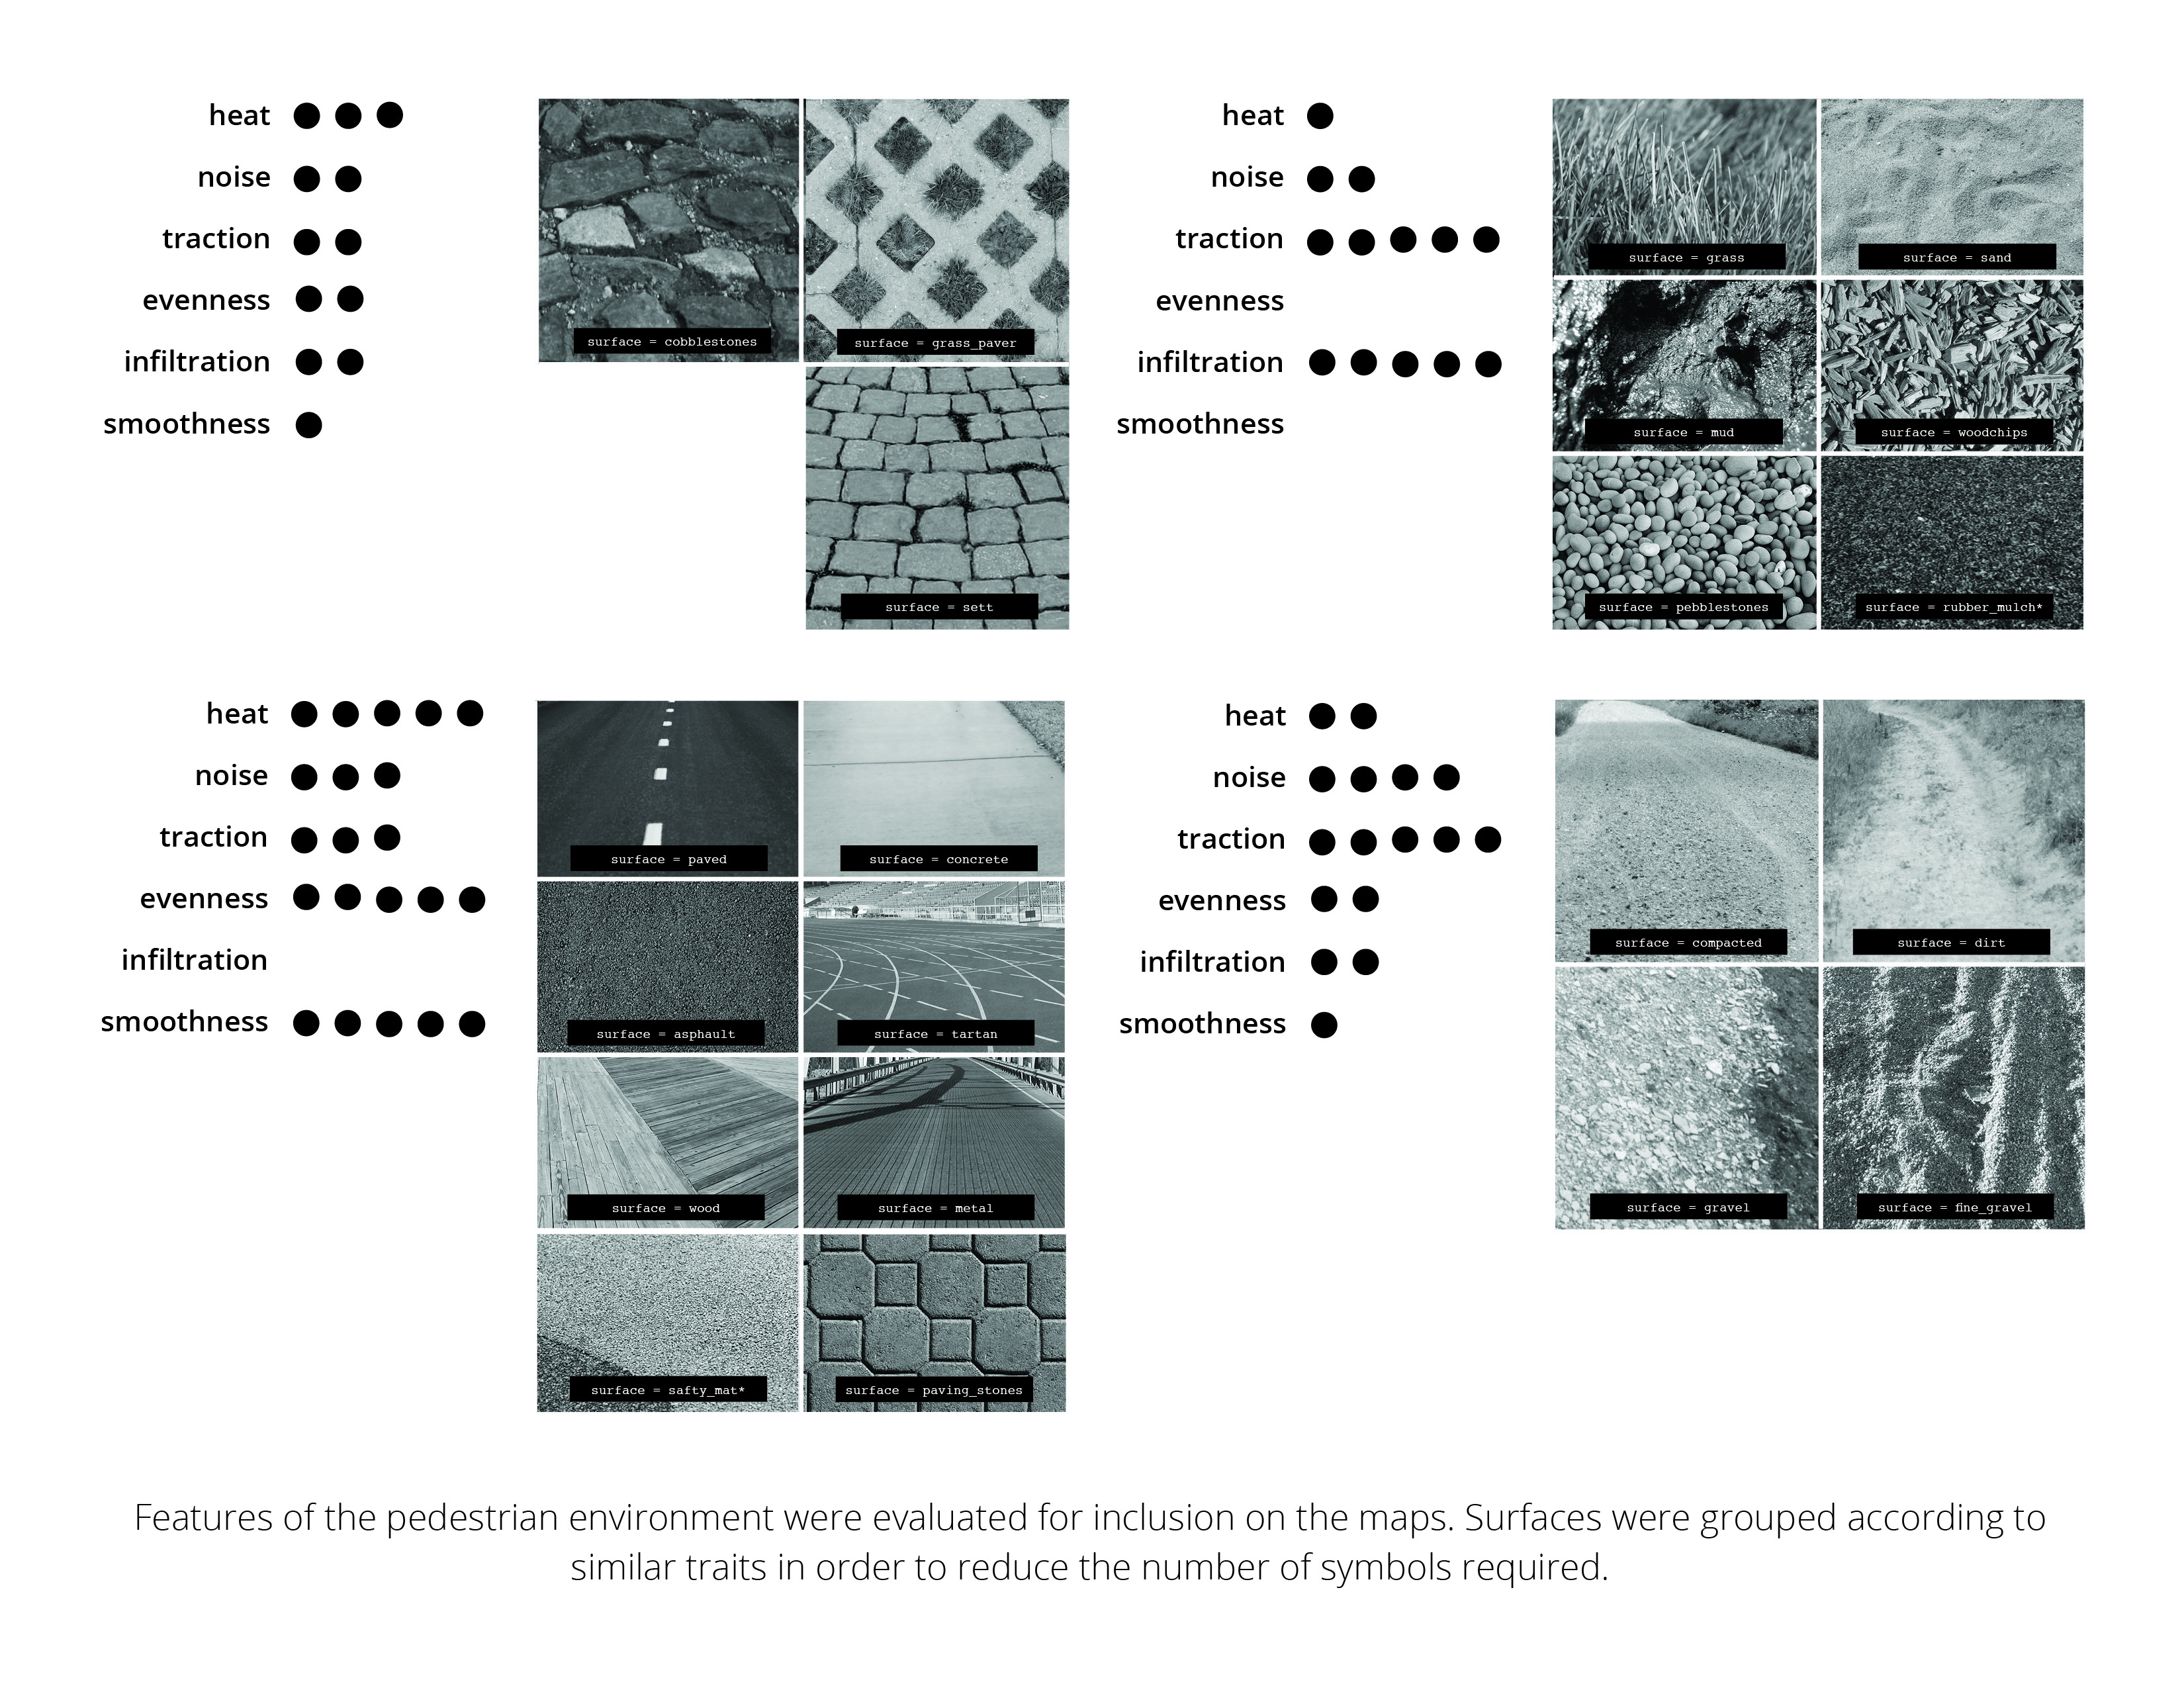
\includegraphics[width=5in]{pics/SidewalkFeatures.jpg}
    \caption{Features of footpath surfaces included in the OpenSidewalks data standard, for inclusion in our tactile maps}
    \label{fig:DataFeatures}
\end{figure}

Appendix \ref{sec:standarddata} includes an overview of features the OpenSidewalks data project collects pertinent to blind, low vision and Deaf-blind pedestrians. As requisite features of any pedestrian environment, surfaces are first explored, followed by topography, which is nearly as ubiquitous.  Street interfaces, while occupying less space in a pedestrian environment, arguably have the greatest impact on pedestrian safety and well-being and are the third feature set considered. 


\subsubsection{Proposed Development}
Only some of the surface features we discuss have been studied in relationship to the experience of visually impaired pedestrians (Secchi, Lauria, and Cellai 2017). 

In this development task, we plan to fully collect all the cartographic features of the OpenSidewalks standards in two pilot areas. This will 
support the development and testing of our Proof of Product application.
We will use the data in the creation of the tactile maps to enable both testing the optimization algorithm we develop (Section \ref{sec:optimize}) and appropriate environments for field studies (Section \ref{test:fieldstudies}). We will be able to better answer several open questions remaining in understanding the use of the standards towards fabricating Tactile Maps with pilot zones in very different environments:
\begin{description}
\item[Downtown Seattle by City Hall] This area contains a significant volume of Seattle's fixed-route bus lines and lightRail transit, including two undergraound stations. The Downtown Seattle Zone will be the testing ground for many important use cases including servicing 
users who take transit to travel to or from a downtown core, with a highly complex geographical topology (many hills) and transit and pedestrian network.
\item[The University of Washington LightRail Station] is a transit transfer center and a park‐and‐ride, along with a hub for hospitals and patient care facilities. The University of Washington Stations 
Zone will be the testing ground for the transfer center use case: a traveler needs to transfer from one transit route to another and must locate the appropriate bus bays within the transit center to complete his or her trip.
\end{description}

\begin{comment}
push this to validation

First, we need to provide a prioritization of the cartographic features from OpenSidewalks as they pertain  ascertain which of the pedestrian cartographic features from OpenSidewalks should be prioritized in tactile maps given that not all could be equally weighted \cite{haberling2008proposed}.
Second, the features we describe may not be appropriate for all map scales or travel purposes.   
Third, our previous tests did not include field testing. 
We ought to offer different weighting for different map purpose (for example, bus stops are not as highly prioritized when users request a map for local exploration, whereas bus stops and their amenities need to be highlighted when a map is requested for a specific transit trip).

\end{comment}



\subsubsection{Validation}

The following validation statements should be tested and hold true if the design goal for this development activity is met: 

Detailed sidewalk layer data is available for all streets in the pilot regions.

Updated transit feed data is available for all streets in the pilot regions.

Here we describe our validation tests for both statements. The data elements and sources are referencing tests and data collection that will occur with our community partners. These data collection activities are described in later sections with greater detail.

\textbf{Validation Statement 1:
Detailed sidewalk layer data is available for all streets in the pilot regions.}

\texttt{Performance Metrics:} 

\texttt{Data Elements \& Sources:}

\texttt{Analysis Procedure:}

\textbf{Validation Statement 2:
Updated transit feed data is available for all streets in the pilot regions.}


\texttt{Performance Metrics:} 

\texttt{Data Elements \& Sources:}

\texttt{Analysis Procedure:}
